\documentclass[12pt,a4paper]{article}
\usepackage[utf8]{inputenc}
\usepackage[french]{babel}
\usepackage[margin=2.5cm]{geometry}
\usepackage{graphicx}
\usepackage{fancyhdr}
\usepackage{titlesec}
\usepackage{hyperref}
\usepackage{pdfpages}
\usepackage{tocloft}
\usepackage{xcolor}
\usepackage{enumitem}

% Configuration des liens
\hypersetup{
    colorlinks=true,
    linkcolor=blue,
    filecolor=magenta,      
    urlcolor=cyan,
    pdftitle={Candidature Parcours Actuariat - Fedi Hmida},
    pdfauthor={Fedi Hmida},
}

% Configuration de l'en-tête et du pied de page
\pagestyle{fancy}
\fancyhf{}
\fancyhead[L]{Candidature Parcours Actuariat}
\fancyhead[R]{Partenariat Université du Mans - Juillet 2025}
\fancyfoot[C]{\thepage}

% Configuration des titres
\titleformat{\section}{\Large\bfseries\color{blue}}{\thesection}{1em}{}
\titleformat{\subsection}{\large\bfseries}{\thesubsection}{1em}{}

% Espacement dans la table des matières
\renewcommand{\cftsecleader}{\cftdotfill{\cftdotsep}}

\begin{document}

% Page de garde
\begin{titlepage}
    \centering
    \vspace*{2cm}
    
    {\Huge\bfseries Dossier de Candidature\par}
    \vspace{1cm}
    {\Large Parcours Actuariat\par}
    \vspace{0.5cm}
    {\large Partenariat avec l'Université du Mans\par}
    \vspace{2cm}
    
    {\LARGE\bfseries FEDI HMIDA\par}
    \vspace{1cm}
    {\large Votre adresse complète\par}
    {\large Votre téléphone\par}
    {\large Votre email\par}
    \vspace{2cm}
    
    {\large Appel à candidature - Juillet 2025\par}
    \vspace{1cm}
    {\large Date de soumission : 1er août 2025\par}
    
    \vfill
    
    {\large Candidature pour l'admission au parcours Actuariat\par}
    {\large en partenariat avec l'Université du Mans\par}
\end{titlepage}

% Table des matières
\tableofcontents
\newpage

% Section 1 : Lettre de motivation
\section{Lettre de Motivation}
\label{sec:lettre}

\subsection{Motivation pour le parcours Actuariat}

\noindent
Fedi Hmida\\
Votre adresse\\
Ville, Code postal\\
Téléphone\\
Email\\

\vspace{1cm}

\noindent
Madame, Monsieur,\\

\vspace{0.5cm}

Je vous écris pour exprimer mon vif intérêt pour le parcours Actuariat proposé en partenariat avec l'Université du Mans pour la promotion de juillet 2025.

\textbf{Parcours académique :}
Titulaire d'un baccalauréat mathématiques obtenu en 2021, j'ai poursuivi mes études par une Licence en Ingénierie des Systèmes Informatiques à l'Institut Supérieur d'Informatique de Mahdia (Université de Monastir, Tunisie) de 2021 à 2024. Actuellement en cycle d'ingénieur en informatique à ESPRIT (2024-2025), mon parcours m'a permis de développer de solides compétences en mathématiques, algorithmique, statistiques et modélisation, disciplines fondamentales de l'actuariat.

\textbf{Motivation pour la reconversion :}
Bien que ma formation initiale soit en informatique, ma passion pour les mathématiques appliquées et l'analyse quantitative m'oriente naturellement vers l'actuariat. Cette formation représente l'opportunité parfaite de combiner mes compétences techniques avec des enjeux économiques et financiers majeurs.

\textbf{Compétences transférables :}
Ma formation en ingénierie informatique m'a doté d'atouts précieux pour l'actuariat :
\begin{itemize}
    \item Maîtrise des outils de modélisation et de simulation
    \item Compétences en programmation et traitement de données
    \item Rigueur analytique et capacité de résolution de problèmes complexes
    \item Aptitude au travail avec de grands volumes de données
\end{itemize}

\textbf{Projet professionnel :}
L'actuariat représente pour moi l'opportunité de contribuer à l'évaluation et à la gestion des risques dans les secteurs de l'assurance, de la finance ou de la consultation, en tirant parti de mes compétences techniques et de ma formation quantitative.

\textbf{Intérêt pour le partenariat :}
Le partenariat avec l'Université du Mans offre une formation d'excellence reconnue par la profession, garantissant un enseignement à la fois théorique et pratique, essentiel pour maîtriser les défis actuels du métier d'actuaire.

Je reste à votre disposition pour tout complément d'information et serais honoré de pouvoir contribuer à cette promotion.

\vspace{1cm}

\noindent
Cordialement,\\
\vspace{1cm}
Fedi Hmida

\newpage

% Section 2 : Curriculum Vitae
\section{Curriculum Vitae}
\label{sec:cv}

\subsection{Informations personnelles}
\begin{itemize}[leftmargin=3cm]
    \item[\textbf{Nom :}] HMIDA
    \item[\textbf{Prénom :}] Fedi
    \item[\textbf{Titre :}] Étudiant en ingénierie informatique
    \item[\textbf{Téléphone :}] +216 93 722 130
    \item[\textbf{Email :}] fedi.hmida@esprit.tn
    \item[\textbf{LinkedIn :}] fedi-hmida
    \item[\textbf{Nationalité :}] Tunisienne
    \item[\textbf{Localisation :}] Tunis, Tunisie
\end{itemize}

\subsection{Profil}
Étudiant passionné en génie logiciel à ESPRIT, titulaire d'une licence en ingénierie informatique, spécialisé dans le développement d’applications mobiles avec Flutter, comme en témoigne le projet SolarFlow App. Compétent en développement web avec Symfony, reconnu pour son esprit proactif et son engagement à fournir des solutions innovantes et efficaces.

\subsection{Formation}
\begin{itemize}
    \item[\textbf{2024-2025 :}] Première année Cycle d'Ingénieur en Informatique - ESPRIT (passage en deuxième année Data Science)
    \item[\textbf{2021-2024 :}] Licence en Ingénierie Informatique - Institut Supérieur d'Informatique de Mahdia, École de Mahdia, Tunisie
    \item[\textbf{2021 :}] Baccalauréat Mathématiques - Tunisie
\end{itemize>

\subsection{Compétences}
\begin{itemize}
    \item \textbf{Développement Mobile :} Flutter, Android Studio, Dart
    \item \textbf{Développement Web :} HTML, CSS, JavaScript, Symfony
    \item \textbf{Intelligence Artificielle et Machine Learning :} YOLO,  Computer Vision (détection d'objets)
    \item \textbf{Bases de Données :} MySQL, SQLite
    \item \textbf{Gestion de Projet :} Scrum, Agile, Scrumban
    \item \textbf{Leadership :} Coordination d'équipe et gestion de projet
\end{itemize}

\subsection{Langues}
\begin{itemize}
    \item \textbf{Anglais :} B2
    \item \textbf{Arabe :} Langue maternelle
    \item \textbf{Français :} B2
\end{itemize}

\subsection{Expérience professionnelle}

\subsubsection{MSign - Stage de Projet de Fin d'Études (Février 2024 - Juin 2024)}
\begin{itemize}
    \item Développement d'un système de contrôle énergétique utilisant des technologies IoT
    \item Construction de l'application SolarFlow en Flutter pour suivre la production d'énergie et gérer les appareils connectés en temps réel
\end{itemize}

\subsubsection{Addinn Group - Stagiaire (Juillet 2023 - Septembre 2023)}
\begin{itemize}
    \item Développement d'un apprentissage profond basé sur YOLO utilisant du code personnalisé pour la détection de dommages de véhicules
    \item Intégration d'IA dans un système de réponse soutenu par l'IA pour le traitement automatisé des réclamations
    \item Construction d'une plateforme multi-véhicules permettant aux utilisateurs de soumettre des réclamations, de télécharger des preuves et de suivre les mises à jour via une interface utilisateur intuitive
\end{itemize}

\subsection{Projets}

\subsubsection{SmartClaim - Application de Réclamation d'Assurance Alimentée par l'IA}
\begin{itemize}
    \item Application basée sur Flutter utilisant un rapport OCR pour la classification des documents et l'extraction de données clés depuis les interfaces
    \item Conception et formation d'un modèle de détection d'objets basé sur YOLO pour localiser les dommages de véhicules
    \item Intégration dans un système de réponse soutenu par l'IA pour le traitement automatisé des réclamations
\end{itemize}

\subsubsection{Onboardify - Plateforme d'Intégration Intelligente des Employés}
\begin{itemize}
    \item Contribution à la conception et au développement d'une plateforme hybride robuste construite avec un environnement interactif et convivial
    \item Mise en œuvre de flux d'intégration personnalisés, d'éléments de gamification, de retours en temps réel et de communication fluide entre les managers et les nouveaux employés
\end{itemize}

\subsubsection{Application SolarFlow}
\begin{itemize}
    \item Développement d'une application mobile conviviale utilisant Flutter pour la surveillance et le contrôle d'appareils alimentés par l'énergie solaire
    \item Activation du suivi de la production d'énergie en temps réel, de l'analyse des services et d'une gestion énergétique efficace
\end{itemize}

\subsection{Activités bénévoles}
\begin{itemize}
    \item \textbf{Trésorier, IEEE ESPRIT Student Branch :} Gestion de la planification financière, de la budgétisation et des dépenses de suivi pour soutenir les activités de la branche
\end{itemize}

\vspace{1cm}

\textbf{CV complet en format PDF :}

% Inclusion du CV complet
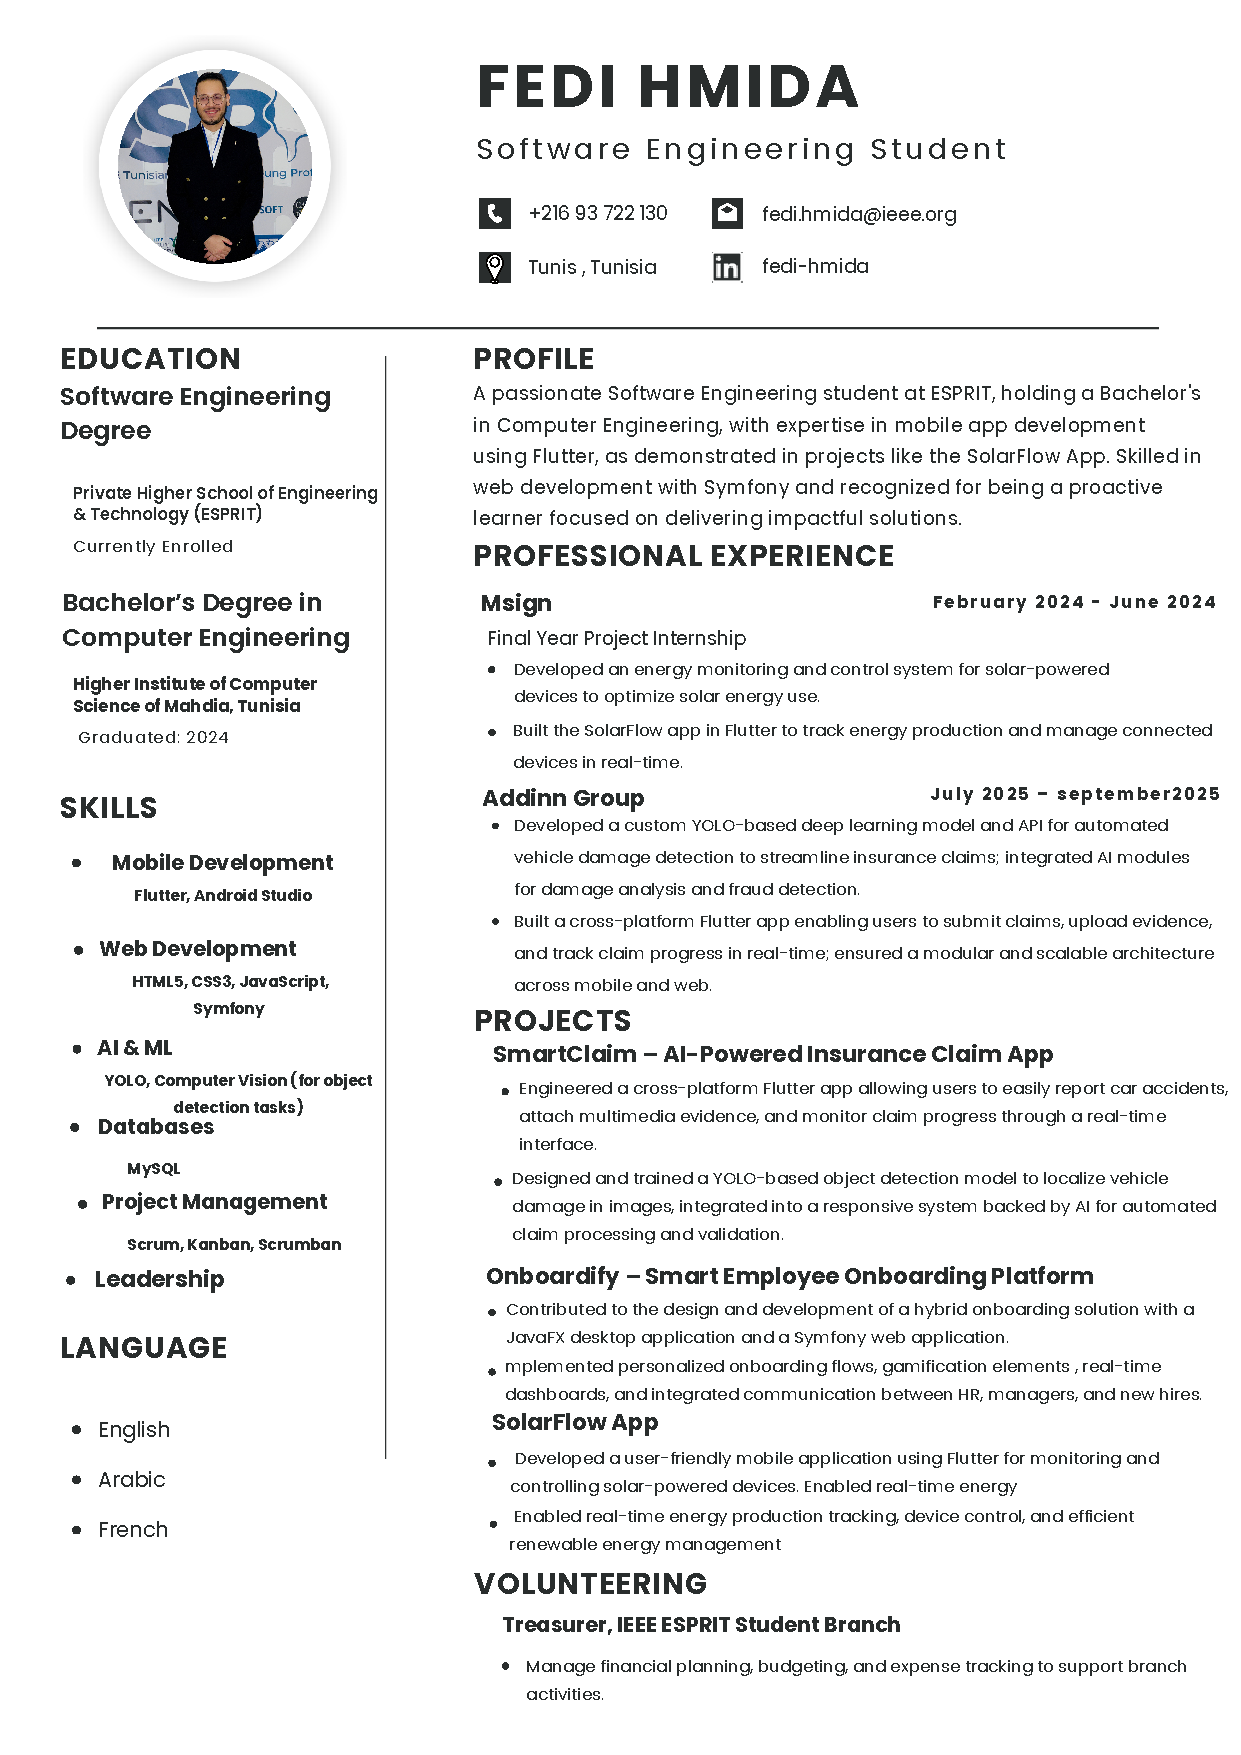
\includepdf[pages=-,pagecommand={\thispagestyle{fancy}}]{CV6.pdf}

\newpage

% Section 3 : Relevés de notes
\section{Relevés de Notes}
\label{sec:releves}

\subsection{Note explicative}
Cette section contient l'ensemble de mes relevés de notes depuis l'obtention du baccalauréat en 2021, présentés par ordre chronologique.

\subsection{Baccalauréat Mathématiques - 2021}
\textbf{Relevé de notes du baccalauréat série Mathématiques obtenu en 2021}

% Inclusion du relevé de notes du bac
\includepdf[pages=-,pagecommand={\thispagestyle{fancy}}]{rélevé notes bac2.0_compressed.pdf}

\subsection{Relevés de notes - Licence en Ingénierie des Systèmes Informatiques}

\textbf{Diplôme obtenu :} Licence en Ingénierie des Systèmes Informatiques

\textbf{Établissement :} Institut Supérieur d'Informatique de Mahdia (ISI Mahdia)

\textbf{Université :} Université de Monastir, Tunisie

\textbf{Années d'études :} 2021 – 2024

\subsubsection{Licence 1 (L1) – Année universitaire 2021–2022}
\textit{Relevé de notes officiel de première année de licence}

\includepdf[pages=-,pagecommand={\thispagestyle{fancy}}]{relevé-de-note-21-22-_compressed.pdf}

\subsubsection{Licence 2 (L2) – Année universitaire 2022–2023}
\textit{Relevé de notes officiel de deuxième année de licence}

\includepdf[pages=-,pagecommand={\thispagestyle{fancy}}]{relevé-de-note-22-23-_compressed[1].pdf}

\subsubsection{Licence 3 (L3) – Année universitaire 2023–2024}
\textit{Relevé de notes officiel de troisième année de licence}

\includepdf[pages=-,pagecommand={\thispagestyle{fancy}}]{relevé-de-note-23-24_-_compressed[1].pdf}

\textit{Copie du diplôme de licence}

\includepdf[pages=-,pagecommand={\thispagestyle{fancy}}]{Diplôme universitaire2.0.pdf}

\subsection{Relevé de notes - Cycle Ingénieur}

\textbf{Formation actuelle :} Cycle d'Ingénieur en Informatique

\textbf{Établissement :} ESPRIT – École Supérieure Privée d'Ingénierie et de Technologies

\textbf{Année universitaire :} 2024 – 2025

\subsubsection{Relevés de notes - Première année de cycle ingénieur}
\textit{Relevé des notes annuelles (2024-2025)}

\textbf{Performances académiques remarquables :}
\begin{itemize}
    \item \textbf{Classement :} 5ème de la classe
    \item \textbf{Moyenne générale :} 13.73/20
    \item \textbf{Projet intégré :} Premier groupe de la classe durant cette année
\end{itemize}

\vspace{0.5cm}

\begin{figure}[h]
    \centering
    \includegraphics[width=0.8\textwidth]{note3.pdf}
    \caption{Relevé de notes annuelles - ESPRIT 2024-2025}
    \label{fig:notes_esprit}
\end{figure}

\newpage

% Section 4 : Rapport de Projet de Fin d'Études
\section{Rapport de Projet de Fin d'Études}
\label{sec:pfe}

\subsection{Page de garde du rapport de PFE}

Ce projet de fin d'études démontre ma capacité à mener un projet technique complexe de bout en bout, compétence essentielle pour la gestion de projets actuariels.

\begin{figure}[h]
    \centering
    \includegraphics[width=0.85\textwidth]{azz.png}
    \caption{Page de garde du rapport de Projet de Fin d'Études}
    \label{fig:pfe_cover}
\end{figure}

\newpage

% Section 5 : Certifications et Attestations
\section{Certifications et Attestations}
\label{sec:certifications}

\subsection{Certifications obtenues}
Cette section présente mes certifications et attestations diverses qui appuient ma candidature.

\subsubsection{Certifications en informatique et mathématiques}
\textit{Listez ici vos certifications pertinentes (programmation, outils statistiques, etc.)}

\subsubsection{Attestations de stage}

\textbf{Attestation de stage de fin d'été}

\begin{figure}[h]
    \centering
    \includegraphics[width=0.8\textwidth]{Stage.png}
    \caption{Attestation de stage de fin d'été}
    \label{fig:attestation_stage}
\end{figure}

\newpage

% Section 6 : Documents complémentaires
\section{Documents Complémentaires}
\label{sec:complementaires}

\subsection{Portfolio de projets}

\textbf{Portfolio complet de mes projets informatiques}

Ce portfolio présente l'ensemble de mes réalisations techniques avec un focus particulier sur les projets ayant des composantes mathématiques et statistiques, démontrant ma capacité à appliquer des concepts quantitatifs dans le développement logiciel.

\begin{figure}[h]
    \centering
    \includegraphics[width=0.9\textwidth]{Portfolio.png}
    \caption{Aperçu de mon portfolio de projets}
    \label{fig:portfolio}
\end{figure}

\vspace{1cm}

\textbf{Lien vers le portfolio complet :}

\href{https://fediportfolio.netlify.app/}{Accéder à mon portfolio en ligne}

\textit{Le portfolio détaille mes projets avec focus sur les applications d'intelligence artificielle, de traitement de données, et de modélisation mathématique, compétences directement transférables vers l'actuariat.}

\newpage

% Section 7 : Conclusion
\section{Synthèse de la candidature}
\label{sec:conclusion}

Ce dossier rassemble l'ensemble des éléments démontrant ma motivation et ma capacité à réussir dans le parcours Actuariat en partenariat avec l'Université du Mans.

\textbf{Points forts de ma candidature :}
\begin{itemize}
    \item Baccalauréat mathématiques (2021) : solide formation quantitative de base
    \item Licence en Ingénierie des Systèmes Informatiques (2021-2024) : compétences techniques et analytiques
    \item Formation actuelle en cycle ingénieur à ESPRIT : approfondissement des compétences
    \item Double compétence mathématiques-informatique, très recherchée en actuariat moderne
    \item Capacités de modélisation et de traitement de données
    \item Motivation claire pour une reconversion vers l'actuariat
\end{itemize}

\textbf{Objectifs professionnels :}
À l'issue de cette formation, je souhaite exercer en tant qu'actuaire en tirant parti de mes compétences techniques pour contribuer à l'innovation dans l'évaluation et la gestion des risques, particulièrement dans les domaines où l'informatique et l'actuariat se rencontrent (InsurTech, modélisation avancée, big data actuariel).

Je reste à votre disposition pour toute information complémentaire et serais honoré de faire partie de cette promotion.

\vspace{2cm}

\noindent
Fedi Hmida\\
1er août 2025

\end{document}